\documentclass[presentation.tex]{subfiles}
\begin{document}
\begin{frame}
\frametitle{STL Intro}
\begin{itemize}
\item Seasonal and Trend decomposition using Loess (STL), as first described by Cleveland et al.
\item Decomposition of a time series ($Y_v$) into a trend ($T_v$), seasonal ($S_v$) and remainder
  ($R_v$) s.t:
  \[
  Y_v = T_v + S_v + R_v \text{ for } v \in 1 \hdots N
  \]
\end{itemize}
\end{frame}

\begin{frame}
  \frametitle{STL Example}
  \begin{figure}[H]
    \centering
    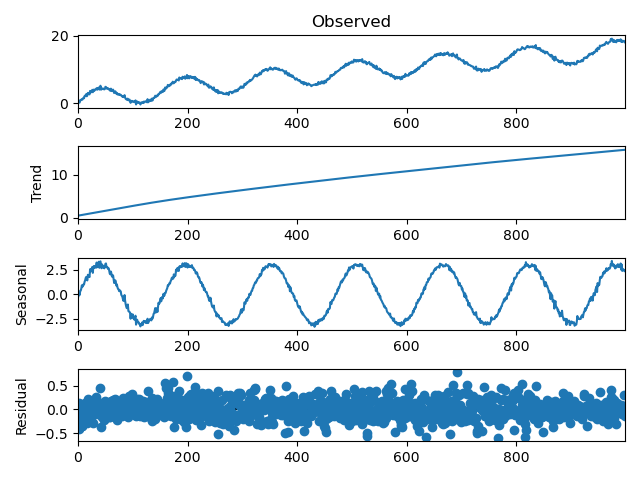
\includegraphics[width=0.7\textwidth]{imgs/stl1.png}
    \caption{$f(x) = x^{0.75} + 2\sin(x)$ with added noise
      $\sim \mathcal{N}(0, 0.25)$}
  \end{figure}
  \centering
\end{frame}


\begin{frame}
\frametitle{Locally Estimated Scatterplot Smoothing (LOESS)}
\begin{itemize}
  \item For all $x$ fit a curve $\hat{g}(x)$ by giving the other points $x_i$ a
  weight $v_i$.
\item Select the value of the smoothing factor $q \in \mathbb{Z}^+$ and let
  $\lambda_q(x)$ be the distance from $x$ to q'th closest $x_i$. For $q > n$:
  \[
  \lambda_q(x) = \frac{q \cdot \lambda_n(x)}{n}
  \]
\item We calculate the weights using the tricube weight function:
  \[
  v_i = \left( 1 - \left( \frac{| x_i - x |}{\lambda_q(x)}  \right)^3\right)^3
  \]
  for $| x_i - x | \geq \lambda_q(x)$, set $v_i = 0$
\item Use locally-linear or locally quadratic fitting with weights
  $\rho_i v_i$, where $\rho_i$ are the robustness weights that make it possible to 
  ignore the outliers in the dataset.
\item The value of $x$ after the application of LOESS is $\hat{g}(x)$,
\end{itemize}
\end{frame}

\begin{frame}
  \frametitle{LOESS Examples}
  \begin{figure}
    \centering
    \begin{subfigure}[b]{0.49\textwidth}
      \centering
      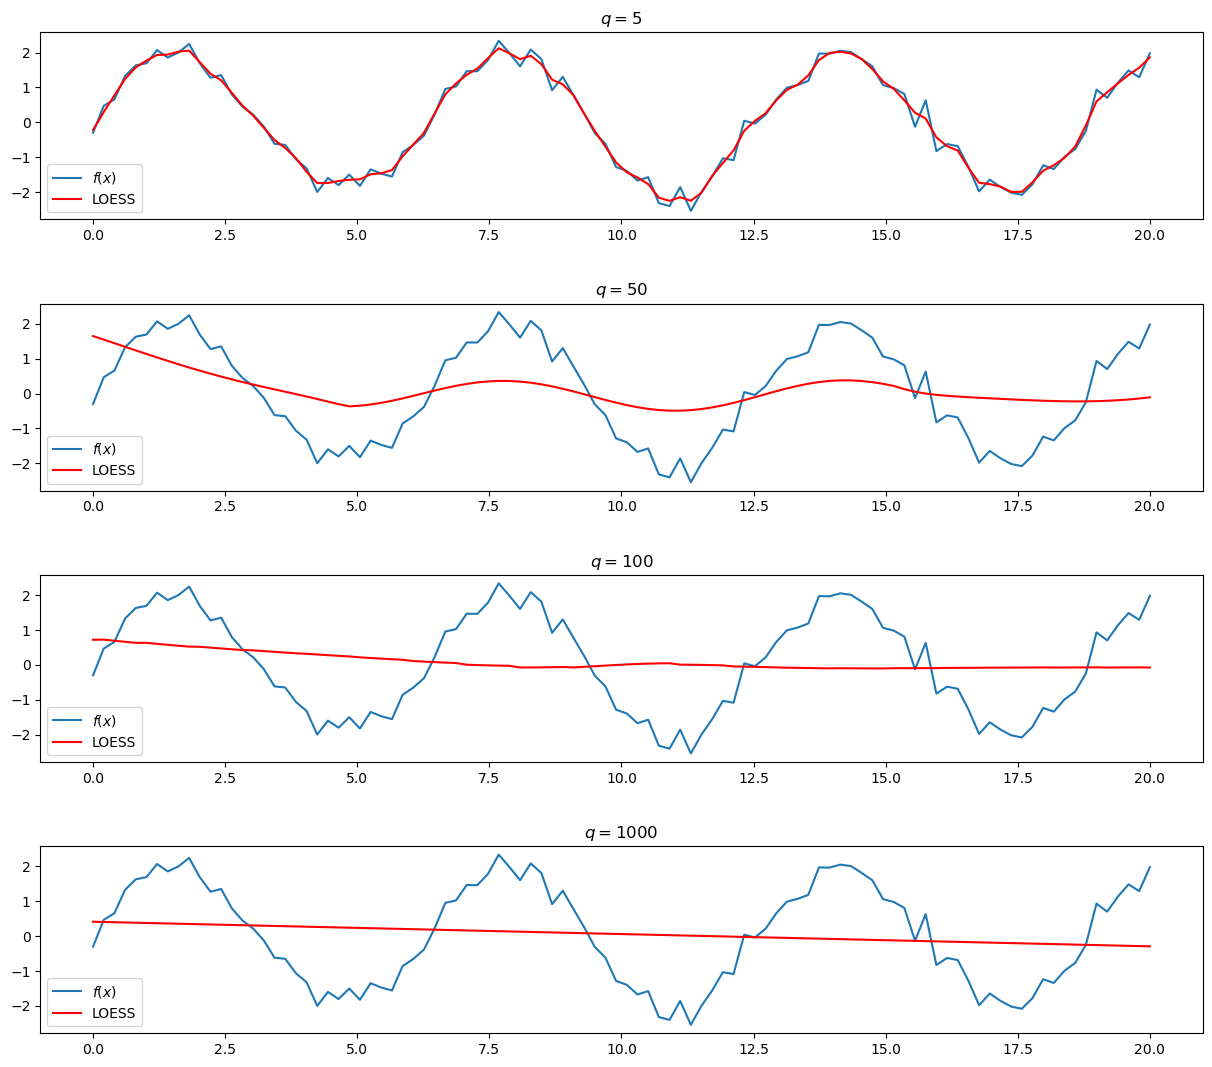
\includegraphics[width=\textwidth]{imgs/loess1}
      \caption{$d=1$}
  \end{subfigure}
  \begin{subfigure}[b]{0.49\textwidth}
    \centering
    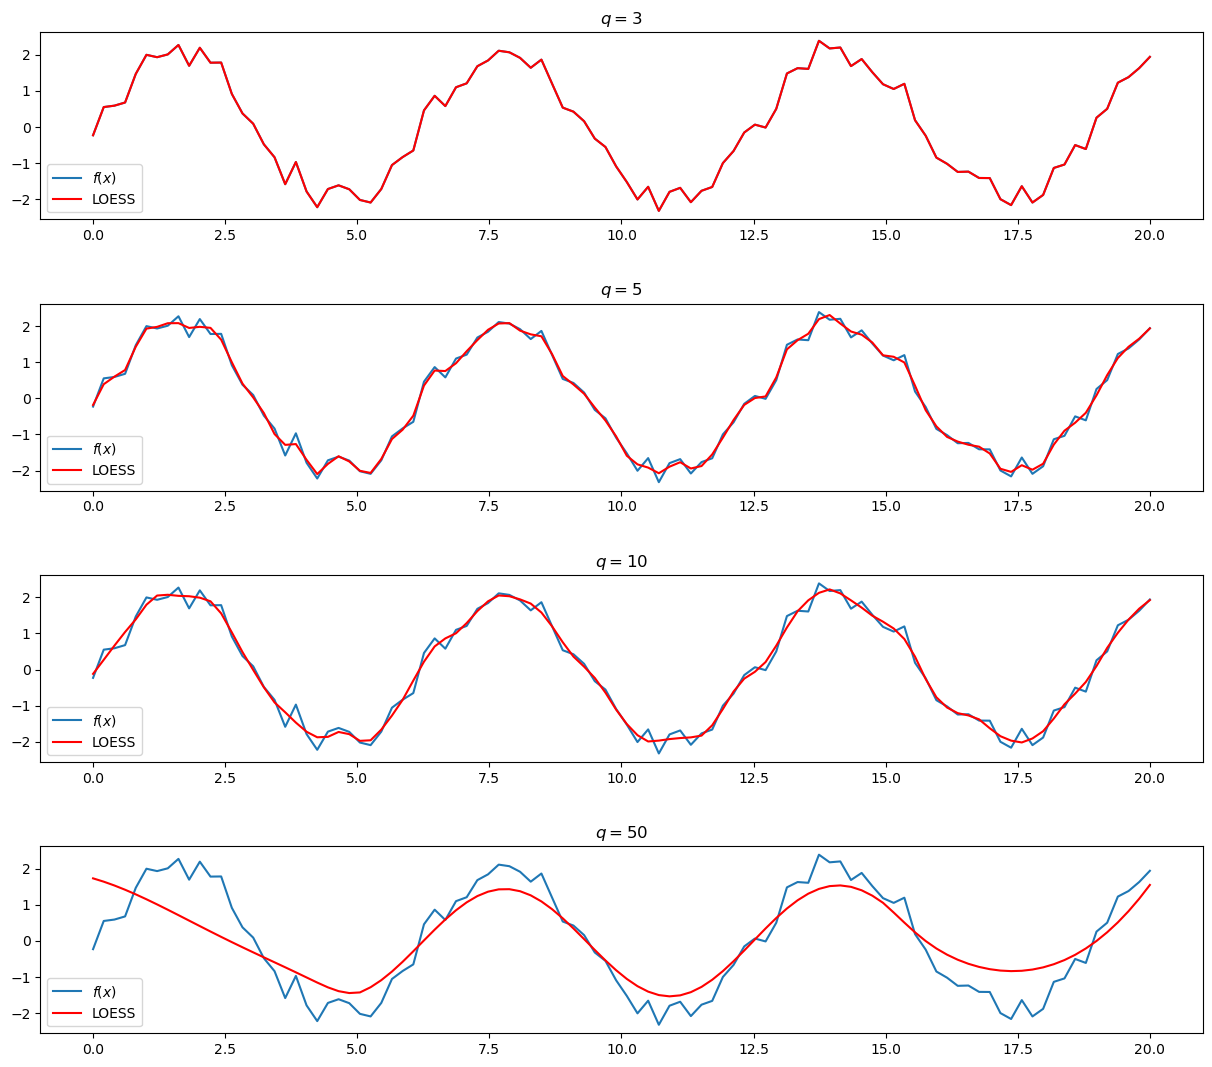
\includegraphics[width=\textwidth]{imgs/loess2}
    \caption{$d=2$}
  \end{subfigure}
  \caption{LOESS applied to $f(x) = 2\sin(x)$ with added Gaussian noise and $n =
    100$. $d$ is the degree of the fitted polynomial, $q$ is the smoothing factor, when
    $q \rightarrow \infty$, LOESS would be equivalent to an ordinary OLS fit of degree $d$}
\end{figure}
\end{frame}

\begin{frame}
  \frametitle{STL - Simplified Algorithm Steps}
  \begin{itemize}
  %% \item STL is performed through two nested loops and we begin by setting:
  \item We begin by setting:
    \[ T_v^{0} = 0, \quad R_v^{0} = 0,  \quad \rho_v = 1 \]
  \item Then for $k$ in $(0, \hdots, n_{\text{iter}}-1)$:
\begin{enumerate}
\item \textbf{Detrending}:
  $V_v = Y_v - T_v^k$, where $k$ is the iteration number of the inner loop
\item \textbf{Cycle-Subseries Smoothing}:
  $V_v$ is split into cycle-subseries, calculate the mean average subseries
  resulting in $C^{k+1}$.
\item \textbf{Low-pass Filter of Smoothed Cycle-Subseries}:
  Apply the low-pass filter to $C_{k+1}$. This is accomplished by application of two
  moving averages of lag equal to 3 followed by LOESS smoothing with $q=n_l$
  and $d=1$. The result is saved as $L^{k+1}$
\item \textbf{Detrending of the Smoothed Cycle-Subseries}:
  $S^{k+1} = C^{k+1} - L^{k+1}$
\item \textbf{Deseasoning}:
  $W_v = Y_v - S_v^{k+1}$. 
\item \textbf{Trend Smoothing}:
  Apply LOESS to $W_v$ with $q = n_t$, resulting in $T^{k+1}$
\end{enumerate}
\item  Return $T^{n_{\text{iter}}}_v$, $S^{n_{\text{iter}}}_v$ and $R^{n_{\text{iter}}}_v = Y_v - T^{n_{\text{iter}}}_v - S^{n_{\text{iter}}}_v$
  \end{itemize}
\end{frame}

%% \begin{frame}
%%   \frametitle{STL - Simplified Algorithm Steps Continued}
%%   \begin{itemize}
%% \item  The outer loop consists of following steps:
%%   \begin{enumerate}
%%   \item Run the inner loop
%%   \item Find the remainder, ($T_v$ and $S_v$ are from the last iteration of the inner loop):
%%     $R_v = Y_v - T_v - S_v$
%%   \item Calculate the robustness weights from the remainder component:
%%     \[
%%     \rho_{v}= B\left( \frac{|R_v|}{6\cdot\text{median}(|R_v|)} \right)
%%     \]
%%     where $B$ is the bisquare weight function:
%%     \[
%%     B(x) =
%%     \begin{cases}
%%       \left(1-x^{2}\right)^{2} & \text{ for } 0 \leqslant x<1 \\
%%       0                     & \text{ for } x>1
%%     \end{cases}
%%     \]
%% \end{enumerate}
%% \item The inner loop is normally ran $2$ times, while the outer loop is ran
%%   once, unless there are outliers present in the dataset.
%% \item Return $T_v$, $S_v$ and $R_v$
%%   \end{itemize}
%% \end{frame}

\end{document}
